\section{Newton und die Kraft}
\label{sec:physik:newton}

\begin{marginfigure}%
    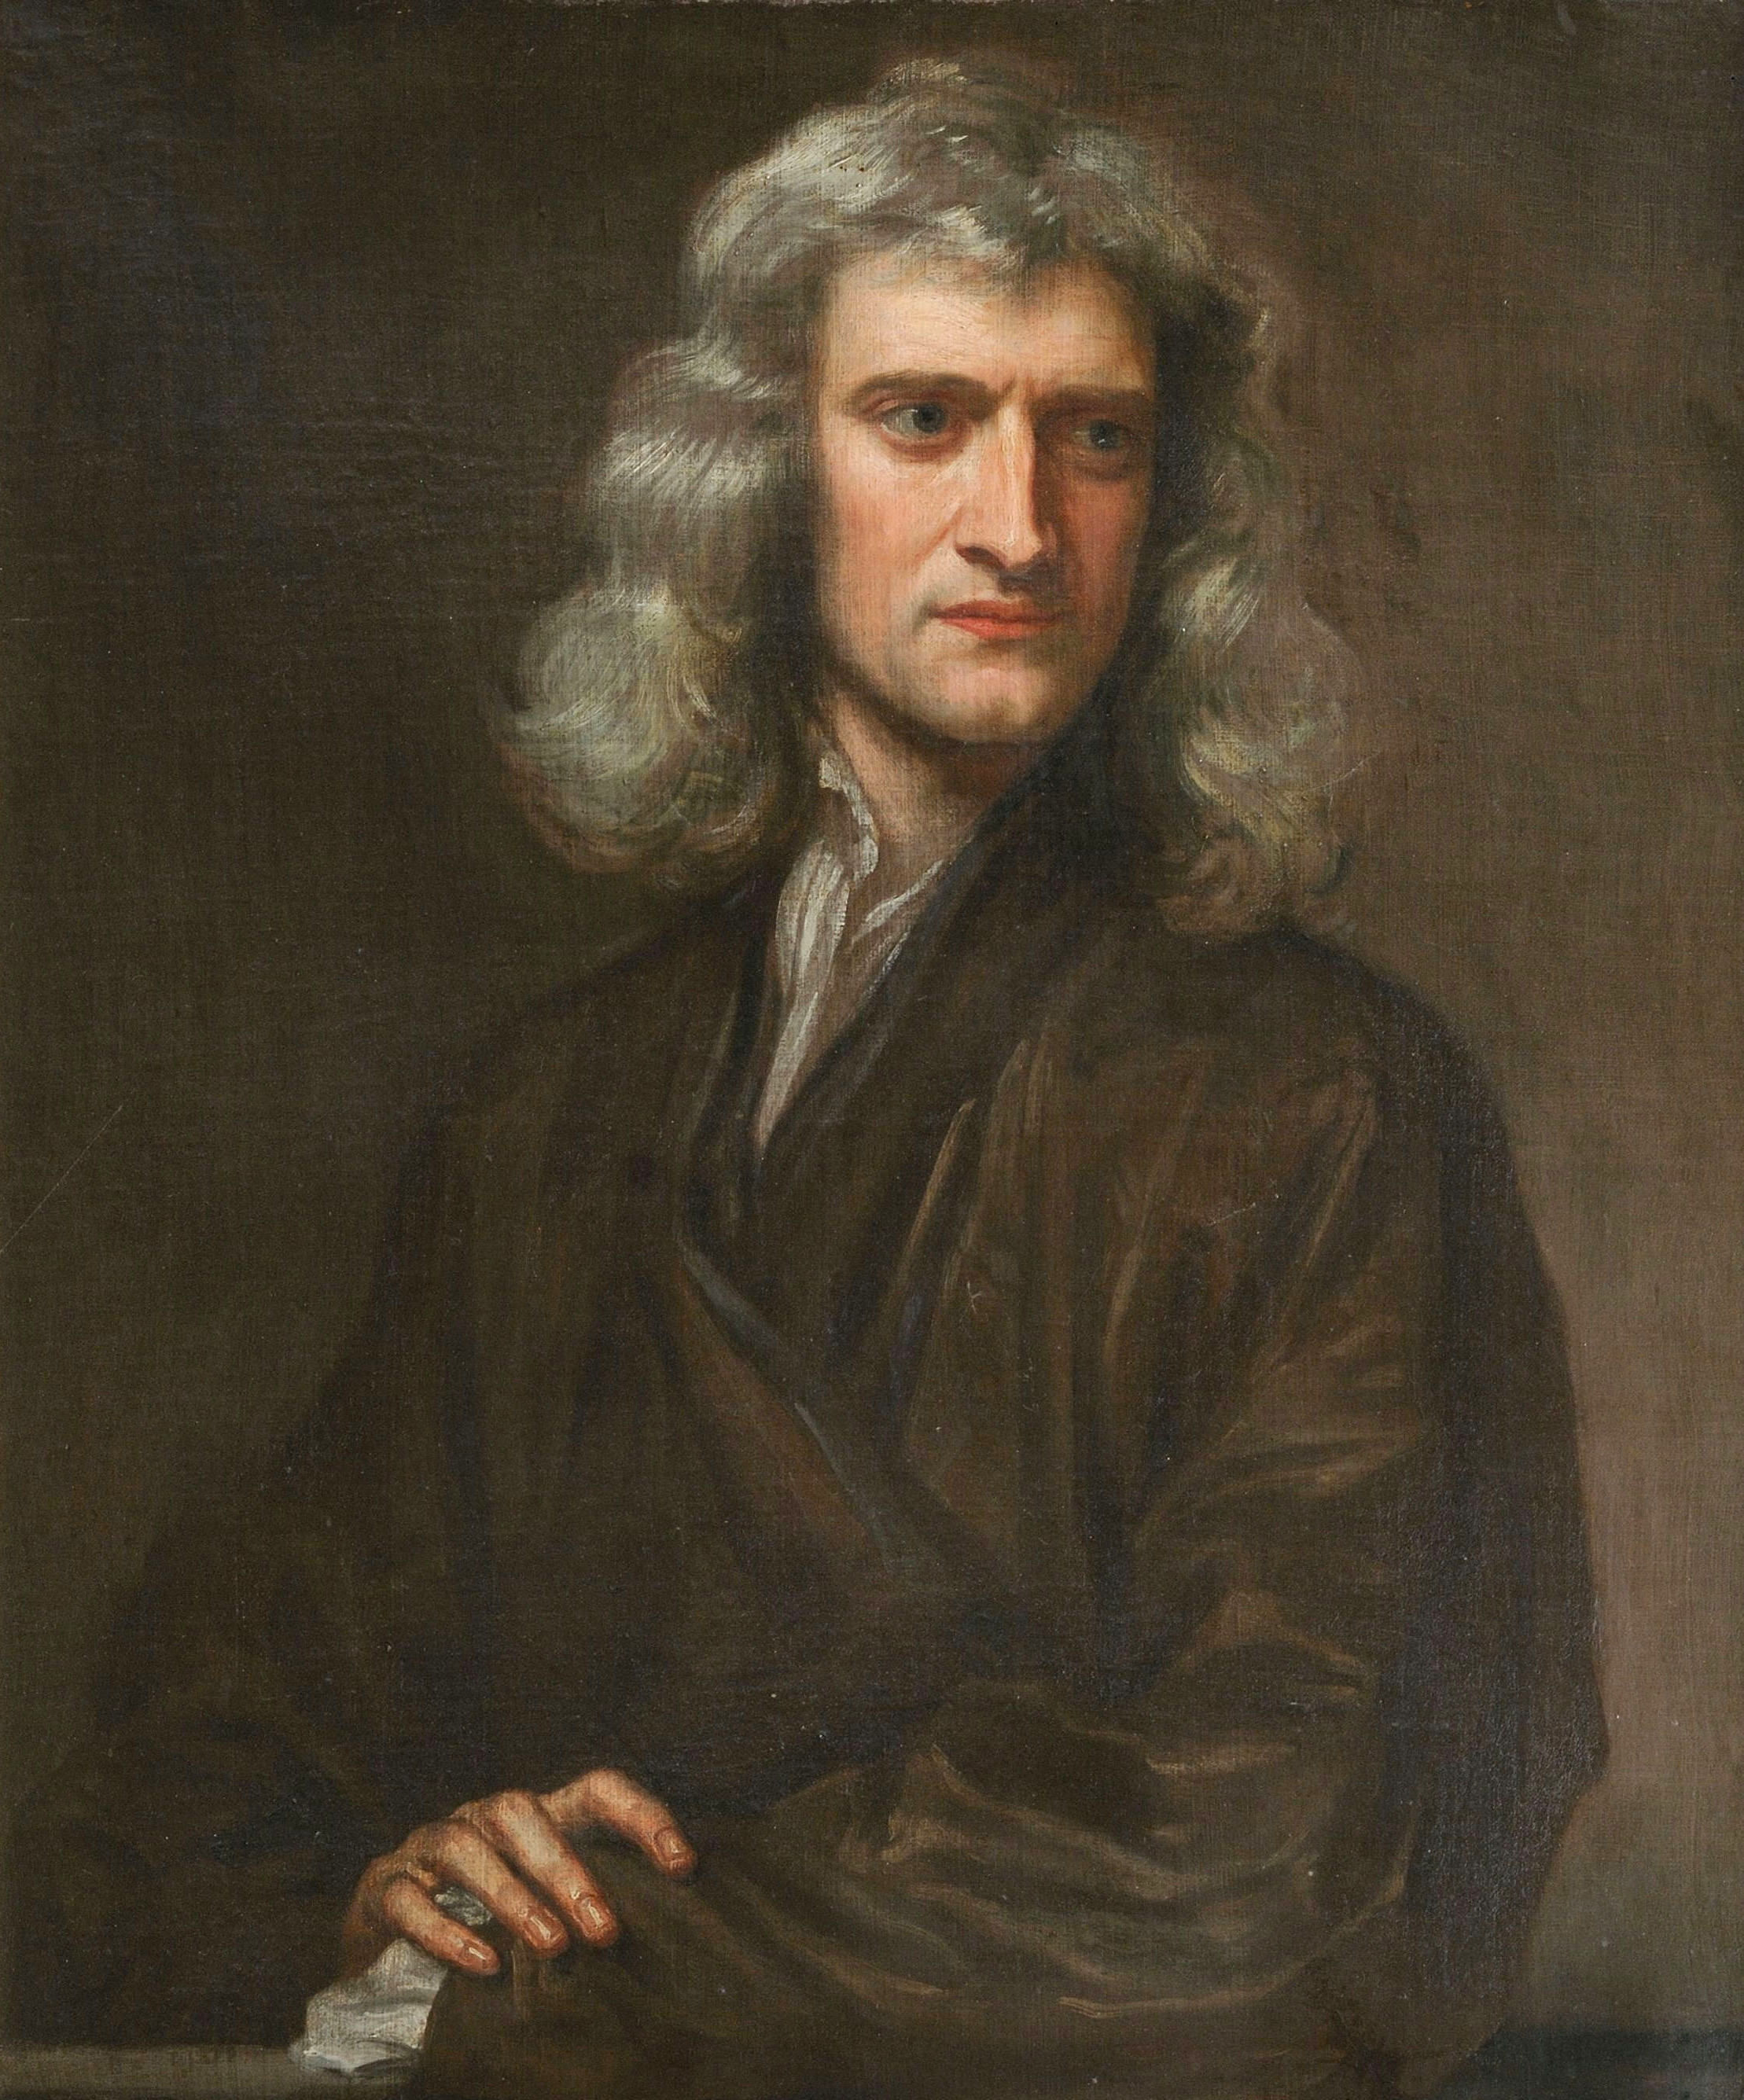
\includegraphics[width=\linewidth]{images/Portrait_of_Sir_Isaac_Newton,_1689_(brightened).jpg}
    \caption{Sir Isaac Newton, 1643--1727. (Gemälde von Godfrey Kneller, 1689. Das Bild ist gemeinfrei / Allgemeingut, Wikimedia Commons)}%
    \label{fig:physik:newton}
\end{marginfigure}%
Sir Newton saß in seinem Garten unter einem Apfelbaum, als er einen Apfel fallen sah. Augenzeugen berichten, dass er tief in Gedanken versunken war. Der fallende Apfel löste eine Gedankenkette aus und er fragte sich: Warum fällt der Apfel immer gerade nach unten -- und warum fällt der Mond nicht auch auf die Erde? Die Schlüsse, die er zog, haben noch immer Gültigkeit. 

Aus diesen Gedanken sind drei Naturgesetze entstanden, die er 1687 veröffentlichte (und noch immer gelehrt werden):
\begin{description}
\item[Trägheit] Ein Körper, auf den keine Kraft wirkt, behält seinen Bewegungszustand bei.
\item[Kraft und Beschleunigung] Kraft ist gleich Masse mal Beschleunigung.
\item[Wechselwirkung] ``actio'' ist gleich ``reactio'' -- Übt ein Körper A auf einen anderen Körper B eine Kraft aus (actio), so wirkt eine gleich große, aber entgegen gerichtete Kraft von Körper B auf Körper A (reactio).
\end{description}
% TODO: add a footnote about the pronounciation of actio and reactio?

\vskip\baselineskip

\noindent
Schauen wir uns die drei Gesetze einmal genauer an:\footnote{%
    FIXME Aristoteles, Descartes, Euler, und so weiter, haben schon vor Newton daran gearbeitet. Übrigens, bis vor 100 Jahren sagte man nicht Physiker, sondern Naturphilosophen... Newton hat als Erster erkannt, dass die Kraft, die einen Apfel fallen lässt, dieselbe ist, die die Planeten bewegt... Streng genommen sind es Axiom...}

\vskip\baselineskip

\noindent
\textbf{Trägheit}\footnote{%
    Das 1.\ Newtonsche Gesetz wird als \textbf{Trägheitsprinzip} bezeichnet.}\\
Den Begriff Trägheit kennt Ihr natürlich Wenn Ihr träge seid (sprich: einfach keine Lust habt, etwas zu tun), bleibt Ihr sitzen und verändert Euren ``Bewegungszustand'' nicht. Aber genau das meint Newton nicht und es ist sehr schwer zu verstehen, weil wir es tatsächlich nicht beobachten können. Was Newton meint, ist, dass ein Körper -- auf den keine Kräfte wirken -- seine Geschwindigkeit beibehält. Auf ein Auto übertragen hieße das: wenn man in der Stadt mit \qty{30}{\km\per\hour} fährt und man den Fuß vom Gas nimmt (der Motor also keine Kraft mehr an die Räder weitergibt) dann fährt das Auto mit \qty{30}{\km\per\hour} bis in alle Unendlichkeit so schnell weiter, bis man die Bremse betätigt. Die Krux\footnote{%
    Krux (von lateinisch \emph{crux}, das Kreuz) bedeutet so viel wie `Schwierigkeit' oder `Haken'. Den Begriff könnt Ihr Euch merken, falls Ihr einmal Scrabble spielt und nicht wisst, was Ihr mit einem 'X' machen sollt.}
daran ist, das wir daran gewöhnt sind, Reibung nicht als ``Kraft'' zu verstehen. Im physikalischen -- und damit Newtons -- Sinn, ist aber Reibung eine Kraft. Bei einem Auto sind das zum Beispiel die Reifen auf der Straße. Aber auch der sogenannte Luftwiderstand, der vor allem für unsere Regensimulation eine Rolle spielt -- und den wir später noch genauer anschauen werden, ist ``Reibung'': eine Kraft. Was Newton also meint: ein Körper, auf den keine Kraft einwirkt (weder Anziehungskraft noch Reibung) bewegt sich \emph{gleichmäßig} weiter (siehe vorhergehendes Kapitel -- $v=0$, also ``stehen bleiben'', gehört dazu). 
% TODO "weil wir es tatsächlich nicht beobachten können" sollte erklärt werden...

\vskip\baselineskip

\noindent
\textbf{Kraft und Beschleunigung}\footnote{%
    Das 2.\ Newtonsche Gesetz wird als \textbf{Aktionsprinzip} bezeichnet.}\\
Vom Fußballspielen wisst Ihr natürlich, dass, wenn Ihr doppelt so stark den Ball tretet, dass der Ball dann auch gefühlt doppelt so weit fliegt. Aber warum ist denn nun die Kraft gleich Masse mal Beschleunigung. 

Denkt mal an eine Feder. Wenn Ihr an einer Feder zieht, verlängert sie sich. Zieht Ihr doppelt so stark, verlängert sie sich doppelt so weit. Eine Feder ist also ein prima Kraftmesser. Hängt man ein Gewicht (zum Beispiel ein 1-kg-Stück) an die Feder, verlängert sie sich um eine bestimmte Strecke. Hängt man zwei gleiche Gewichte daran, verlängert sie sich doppelt so weit. Die Gewichte ziehen also doppelt so stark an der Feder.

Jetzt stellen wir uns vor, wir fliegen zum Mond. Dort ist die Anziehungskraft nur ein Sechstel so groß wie auf der Erde. Was beobachten wir? Die Feder verlängert sich nur noch ein Sechstel so weit. Das Gewicht zieht also nur noch ein Sechstel so stark.

Was passiert nun, wenn wir das Gewicht fallen lassen? Auf dem Mond fällt es sechs Mal langsamer zu Boden als auf der Erde. Die Beschleunigung ist also auch nur ein Sechstel so groß -- und jetzt kommt der Trick: Was gleich bleibt, ist die Masse! Denn Ihr nehmt ja nichts von den Gewichten weg und tut auch nichts hinzu. Das Verhältnis von Kraft zu Beschleunigung bleibt also gleich. Genau das steckt in der Formel $F=m\cdot a$: die Kraft ist das Produkt aus Masse und Beschleunigung. 

(Und dass ein Hammer und eine Feder im Vakuum sogar gleich schnell fallen, obwohl sie unterschiedlich schwer sind -- das schauen wir uns später bei der Reibung an.)

\begin{challenge}
    Die Einheit der Kraft ist $\mathrm{N}$, das heißt tatsächlich ``Newton''. Die Erdbeschleunigung ist $g = \qty{9,81}{\meter\per\second^2}$. Wenn man nur eine Abschätzung haben will, nimmt für den Wert einfach gerundet eine $10$. Mit der Formel $F=m\cdot a$ ($a$ ist die Beschleunigung, dafür nehmen wir jetzt die Erdbeschleunigung $g$) heißt das: ein Gewicht von \qty{1}{\kg} wird mit etwa \qty{10}{\N} von der Erde angezogen.
    \begin{enumerate}[label=\roman*)]
        \item Rechnet aus, mit groß Eure Gewichtskraft ist.
        \item Ein kleiner Tropfen wiegt ungefähr \qty{0.1}{\g}. Wie hoch ist die Kraft, mit der er von der Erde angezogen wird? (Vorsicht, hier steht nicht ``Kilogramm''!)
        \item Das Triebwerk eines modernen Linienflugzeugs erzeugt einen Schub von \qty{30}{\kilo\N}. Wie groß ist die Masse, die einer Gewichtskraft von \qty{350}{\kilo\N} entsprechen würde?
    \end{enumerate}
    \begin{solution}
        \begin{enumerate}[label=\roman*)]
            \item Der Autor wiegt \qty{75}{\kg} und hat damit eine Gewichtskraft von ungefähr \qty{750}{\N}.
            \item Ein Tropfen mit einer Masse von \qty{0.1}{\g} wird mit \qty{1}{\milli\N} zur Erde beschleunigt (das ``m'' vor dem N steht für ``milli'' -- Ihr kennt das hoffentlich von Milliliteren, geschrieben ``mL'' oder ``ml'').
            \item Der Schub des Triebwerks entspricht der Gewichtskraft einer Masse von \qty[exponent-mode=fixed]{35000}{\kg}. Zum Vergleich: ein A380 wiegt leer ungefähr das zehnfache dieses Wertes.  
        \end{enumerate}
    \end{solution}
\end{challenge}
% TODO: add a figure describing the relation of unit N to kg (rope over the edge of a table with a weight pulling something horizontally)?


\vskip\baselineskip

\noindent
\textbf{Wechselwirkung}\footnote{%
    Das 3.\ Newtonsche Gesetz wird als \textbf{Wechselwirkungsprinzip} bezeichnet}\\
Ihr könntet Euch jetzt fragen: wenn wir auf der Erde stehen und die Erde eine Gewichtskraft auf mich ausübt, übe ich dann auch die gleich Kraft auf die Erde aus? Die Antwort ist kaum zu glauben: Ja! Es wird sogar noch unglaublicher: Wenn Ihr von der Erde wegspringt, beschleunigt Ihr nicht nur Euch selbst, sondern auch die Erde mit der gleichen Kraft, mit der Ihr losgesprungen seid.\footnote{%
    Falls Ihr Euch fragt, ob man das Messen könnte, dann müsst Ihr wissen, dass die Erde ungefähr eine Masse von \qty{6e24}{\kg} hat -- das ist die Zahl 6 mit 24 Nullen. Selbst wenn alle Menschen sich auf einer Seite der Erde zusammenfinden und gleichzeitig hochspringen, ist das Verhältnis so enorm, dass man es nicht feststellen könnte.}

Am besten kann man sich dieses Wechselwirkungsprinzip vorstellen, in dem wir uns fragen, wie eine Rakete zum Mond fliegen kann. Eine Rakete ist tatsächlich nichts anderes als ein riesiger Motor, der heiße Gase mit voller Wucht nach unten ausstößt. Die Kraft, mit der die Gase ausgestoßen werden (actio), drücken die Rakete mit derselben Kraft in die entgegengesetzte Richtung (reactio). Die Rakete muss also gar nicht an etwas ``ziehen'', um nach oben zu kommen -- sie erreicht das, indem sie etwas nach unten wirft. Der Ausstoß muss allerdings so groß sein, dass die Rakete auch der Erdanziehung ``entfliehen'' kann. Ohne dieses Gesetz (das man deshalb auch das Rückstoßprinzip nennt) wäre die Menschheit nie in den Weltraum gekommen.

